\documentclass{article}
\usepackage{graphicx} % new way of doing eps files
\usepackage{listings} % nice code layout
\usepackage[usenames]{color} % color
\usepackage{float}
\definecolor{listinggray}{gray}{0.9}
\definecolor{graphgray}{gray}{0.7}
\definecolor{ans}{rgb}{1,0,0}
\definecolor{blue}{rgb}{0,0,1}
% \Verilog{title}{label}{file}
\newcommand{\Verilog}[3]{
  \lstset{language=Verilog}
  \lstset{backgroundcolor=\color{listinggray},rulecolor=\color{blue}}
  \lstset{linewidth=\textwidth}
  \lstset{commentstyle=\textit, stringstyle=\upshape,showspaces=false}
  \lstset{frame=tb}
  \lstinputlisting[caption={#1},label={#2}]{#3}
}


\author{Jiasen Zhou, Jon Johnston}
\title{Lab 12: Pipeline Fetch and Decode}

\begin{document}
\maketitle

\section{Executive Summary}
The goal of this lab was to pipeline the Fetch and Decode stages of the finished datapath. The Execute, Memory, and Writeback stages are commented out to isolate the Fetch and Decode stages of the datapath. The pipeline buffers between the stages are added so that the datapath stil operated correctly. Some additional registers are added to demonstrate the future operation of the pipeline. The lab is successful, and the Fetch and Decode stages of the datapath are now pipelined.

\section{Test Report}
To verify operation of these modules, this lab required one test bench. 
\begin{enumerate}
	\item Pipeline Test Bench
\end{enumerate}

\subsection{Pipeline Test Bench}
The Pipeline Test Bench contains:
\begin{enumerate}
	\item Inputs
	\begin{enumerate}
		\item branch\_target - branch address
		\item pc\_src - the control of branch mux
		\item reset - set the current pc to be 0
										
	\end{enumerate}	
	\item Outputs
	\begin{enumerate}	
		\item uncond\_branch\_id, branch\_id, mem\_read\_id, mem\_to\_reg\_id, mem\_write\_id, ALU\_src\_id, reg\_write\_id, ALU\_op\_id, opcode\_id, read\_data1\_id, read\_data2\_id, sign\_extended\_output\_id, cur\_pc\_id  - control signals that stored in buffer 
	\end{enumerate}		
		
		The pipelined datapath takes the standard ten instructions and runs them through the Fetch and Decode stages to ensure that the correct values are being operated on in each stage. Operation of the testbench
		is verified by comparing the Simulation Results with the Expected Results Table. The pipelined Fetch and Decode stages operate as expected.

\end{enumerate} 

\pagebreak

\begin{figure} [H]
	\begin{center}
		\caption{Pipeline Buffer Table.}\label{fig:ert_pipelinetable}
		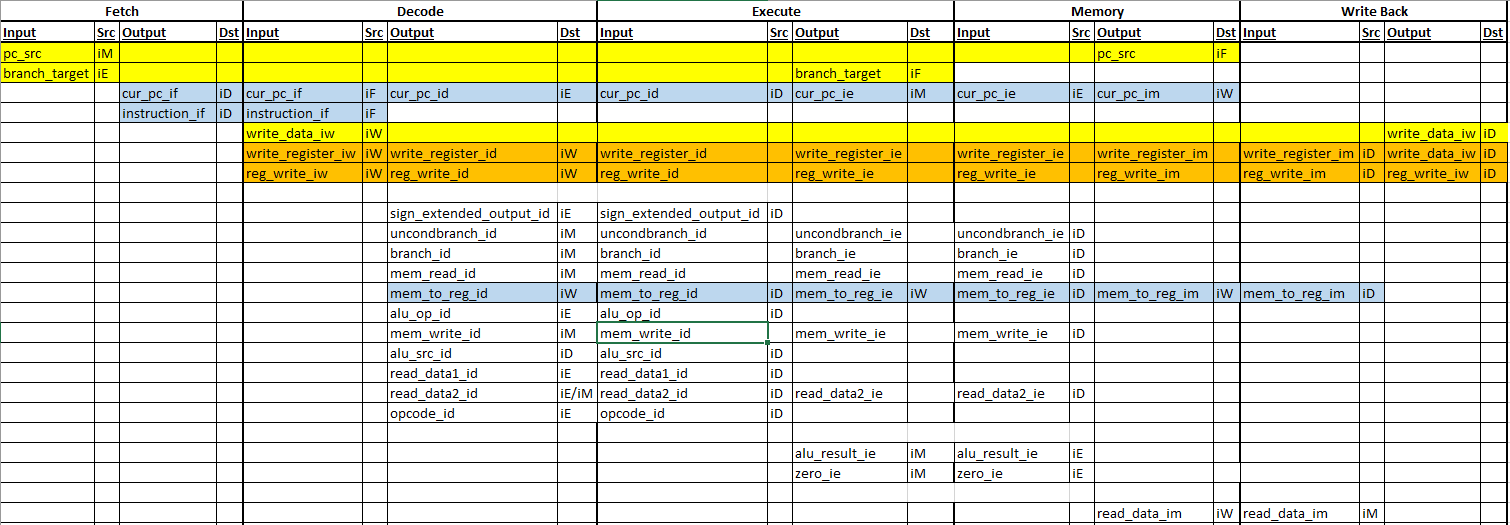
\includegraphics[width=1.0\textwidth]{../images/Lab12_pipelined_datapath_table.PNG}
	\end{center}

	\begin{center}
		\caption{Expected Results Table.}\label{fig:ert_pipelinetable}
		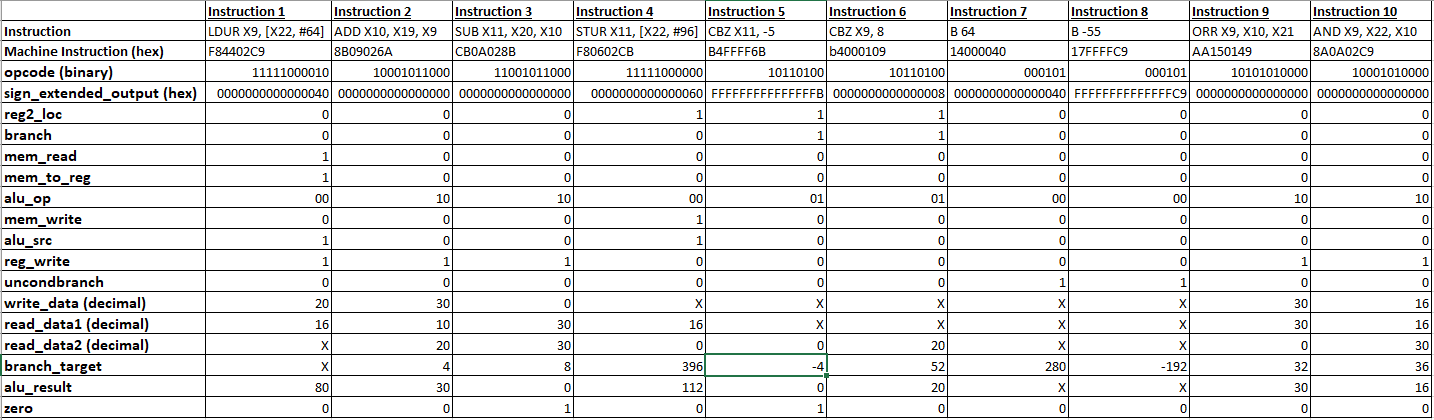
\includegraphics[width=1.0\textwidth]{../images/Lab12_expected_results.PNG}
	\end{center}

	\begin{center}
		\caption{Timing Diagram of the Pipeline test.}\label{fig:ert_pipelinetest}
		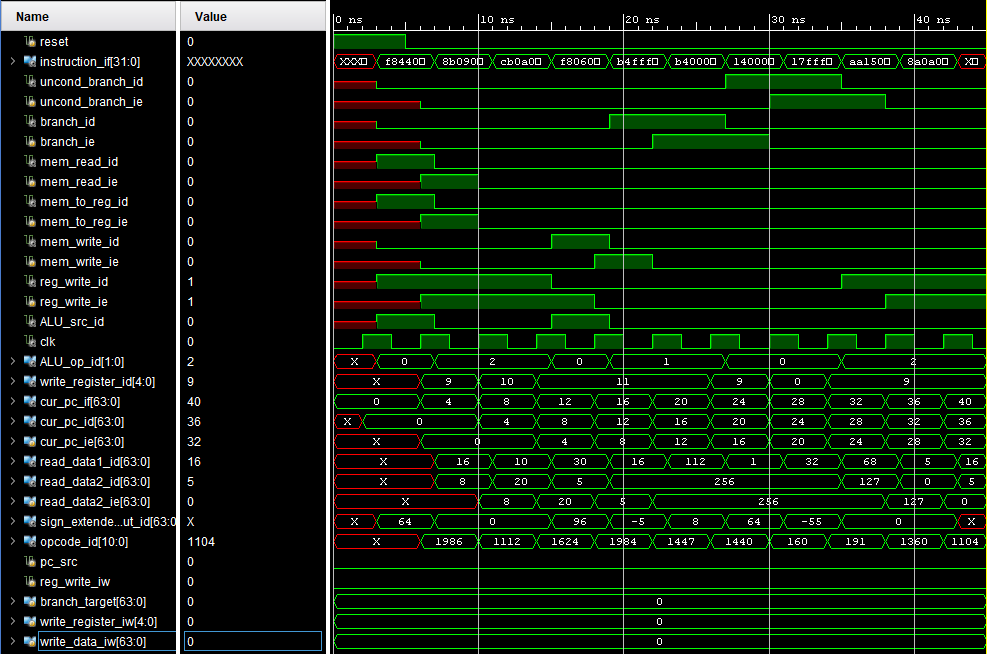
\includegraphics[width=1.0\textwidth]{../images/Lab12_pipelined_datapath_simulation.PNG}
	\end{center}
\end{figure}

\pagebreak
\section{Code Appendix}
% The code appendix should include the test bench code and module code for this lab.
\Verilog{Verilog code for testing the pipelined datapath}{code:pipelinetest}{../code/2_decode/pipeline_datapath.v}

\end{document} 